
\documentclass[12pt]{article}

\usepackage[utf8]{inputenc}
\usepackage[greek, english]{babel}

% Packages
\usepackage{alphabeta}
\usepackage{amsmath}
\usepackage{amsthm}
\usepackage{caption}
\usepackage{color}
\usepackage{float}
\usepackage{fullpage}
\usepackage{graphicx}
\usepackage{hyperref}
\usepackage{latexsym}
\usepackage{listings}
\usepackage{pxfonts}
\usepackage{stackrel}
\usepackage{subfig}
\usepackage{tikz}
\usepackage{titlesec}
\usepackage[ruled,vlined]{algorithm2e}

% Commands
\newcommand{\N}{\mathbb{N}}
\newcommand{\R}{\mathbb{R}}
\newcommand{\abs}[1]{\left\lvert#1\right\rvert}
\newcommand{\code}[2]{\lstinputlisting[caption={#2}]{#1}}
\newcommand{\margin}{\hspace{4pt}}
\newcommand{\norm}[1]{\left\lVert#1\right\rVert}
\newcommand{\argmin}{\operatornamewithlimits{argmin}}
\newcommand{\argmax}{\operatornamewithlimits{argmax}}

% Environments
\newenvironment{matlab}
	{\begin{figure}[H]\centering\captionsetup{justification=centering}}
	{\end{figure}}

\newenvironment{rcases}
	{\left.\begin{aligned}}
	{\end{aligned}\right\rbrace}

% Python Syntax Highlighting
\definecolor{string_color}{RGB}{0, 161, 13}
\definecolor{comment_color}{RGB}{46, 46, 46}
\definecolor{keyword_color}{RGB}{0, 112, 191}
\definecolor{background_color}{RGB}{250, 250, 250}

\lstset{
    framesep=15pt,
    xleftmargin=15pt,
    xrightmargin=15pt,
    language=Python,
    captionpos=b,
    numbers=right,
    numberstyle=\small\ttfamily,
    frame=lines,
    showspaces=false,
    showtabs=false,
    breaklines=true,
    showstringspaces=false,
    breakatwhitespace=true,
    commentstyle=\color{comment_color}\textit,
    keywordstyle=\bfseries\color{keyword_color}\textbf,
    stringstyle=\color{string_color}\textit,
    morekeywords={self, lambda, __init__, __del__, __name__, for, in, not, and, or, :},
    basicstyle=\small\ttfamily,
    tabsize=4,
    keepspaces=true,
    columns=flexible,
    backgroundcolor=\color{background_color}
}

% Links
\hypersetup{
    colorlinks=true,
    linkcolor=blue,
    filecolor=magenta,
    urlcolor=cyan,
}

% Lengths
\setlength{\parindent}{0in}
\setlength{\oddsidemargin}{0in}
\setlength{\textwidth}{6.5in}
\setlength{\textheight}{10in}
\setlength{\topmargin}{-1.0in}
\setlength{\headheight}{18pt}

\titlespacing*{\subsection}
{0pt}{5.5ex plus 1ex minus .2ex}{4.3ex plus .2ex}

\title{\hugeΥπολογιστική Γεωμετρία\\Δεύτερη Εργασία}
\author{Σιώρος Βασίλειος - 1115201500144\\Ανδρινοπούλου Χριστίνα - 1115201500006}
\date{Απρίλιος 2020}

\begin{document}

\maketitle

\pagenumbering{gobble}

\pagebreak


\subsection*{1.Implement from scratch the k-NN algorithm in python programming language.
	Present your method and how you worked, conclude by discussing the disadvantages of the k-
	NN algorithm, if any.}

\subsubsection*{Thought Process and Theory}

Πολύ συχνά, σε διάφορους τομείς της επιστήμης, αλλά και της καθημερινότητας, χρειάζεται να προβλέψουμε συμπεριφορές βασιζόμενοι σε ήδη γνωστά στοιχεία. Ένα τέτοιο πολύ απλό παράδειγμα μπορεί να είναι η πρόβλεψη του βαθμού των φοιτητών στο μάθημα της Υπολογιστικής Γεωμετρίας με βάση τους βαθμούς των φοιτητών των προηγούμενων χρόνων. Στο παράδειγμα αυτό έχουμε ένα σύνολο φοιτητών για τους οποίους γνωρίζουμε τη βαθμολογία τους στο μάθημα (φοιτητές προηγούμενων χρόνων) και ένα σύνολο φοιτητών (φοιτητές τρέχοντος εξαμήνου) για τους οποίους θέλουμε να προβλέψουμε τον βαθμό που θα πάρουν. Η μηχανική μαθηση και η εξόρυξη δεδομένων διαχειρίζεται τέτοια προβλήματα, ανεξάρτητα από τη φύση τους, μέσα από συγκεκριμένους αλγορίθμους. Ένας τέτοιος αλγόριθμος είναι ο αλγόριθμος των κ-πλησιέστερων γειτόνων. \\
 
Ο αλγόριθμος των κ-πλησιέστερων γειτόνων (k-Nearest Neighbor - k-NN) είναι ένα κλασσικός αλγόριθμος μηχανικής μάθησης. Η βασική ιδέα του αλγορίθμου αυτού είναι η πρόβλεψη της κατηγορίας ενός αντικειμένου με βάση τις κατηγορίες αντικειμένων που είναι ήδη γνωστές στον αλγόριθμο. Πιο συγκεκριμένα, ο k-NN έχει να διαχειριστεί δύο διαφορετικά σύνολα αντικειμένων, εκείνα τα αντικείμενα για τα οποία γνωρίζει την κατηγορία (label) στην οποία ανήκουν και εκείνα για τα οποία αγνοεί πλήρως την κατηγορία στην οποία εντάσσονται και επιχειρεί να την προβλέψει. \\

Κάθε αντικείμενο περιγράφεται από ένα σύνολο χαρακτηριστικών. Χαρακτηριστικό καλείται μία ιδιότητα ή ένα γνώρισμα ενός αντικειμένου. Η ιδιότητα (ή το γνώρισμα) μπορεί να παρουσιάζει διαφοροποιήσεις από αντικείμενο σε αντικείμενο ή από χρονική στιγμή σε χρονική στιγμή. Ενδεικτικά, για την περιγραφή του αντικειμένου "άνθρωπος" σε ένα πρόβλημα βιοϊατρικού χαρακτήρα μερικά από τα χαρακτηριστικά που θα το περιέγραφαν μπορούν να είναι: το φύλο, η ηλικία, το βάρος, οι ασθένειες από τις οποίες πάσχει, οι ασθένειες από τις οποίες πάσχουν/έπασχαν οι συγγενείς του, το είδος διατροφής κ.α.. Το πλήθος των χαρακτηριστικών καθορίζει τον χώρο στον οποίον ζουν τα αντικείμενα. Αν για παράδειγμα τα αντικείμενα περιγράφονται από τρία χαρακτηριστικά, τότε τα αντικείμενα εντόπίζονται στον \(\R^3\) και μπορούν να αναπαρασταθούν ως σημεία στον τρισδιάστατο χώρο με x, y και z συντεταγμένη που να αντιστοιχούν στο πρώτο, δεύτερο και τρίτο χαρακτηριστικό αντίστοιχα. Αν τα χαρακτηριστικά δεν έχουν αριθμητική μορφή μπορούν, ανάλογα με τη φύση του χαρακτηριστικού, να μετατραπούν σε αριθμούς.  \\

Επίσης, κάθε αντικείμενο ανήκει σε μία συγκεκριμένη κατηγορία (label). Στο παραπάνω παράδειγμα βιοϊατρικής φύσης η κατηγοριποίηση των ανθρώπων μπορεί να γίνει με βάση την ύπαρξη ή όχι κάποιας συγκεκριμένης ασθένειας σε κάθε άνθρωπο. Συνεπώς, η κατηγορία εδώ είναι "πάσχει/δεν πάσχει" από μία ασθένεια, έστω καρκίνος. \\

Τα χαρακτηριστικά, όπως αναφέραμε προηγουμένως, χρησιμοποιούνται για να περιγράψουν το εκάστοτε αντικείμενο και είναι συνυφασμένα με την κατηγορία στην οποία εντάσσεται το αντικείμενο με τέτοιον τρόπο ώστε αντικείμενα που μοιάζουν μεταξύ τους να ανήκουν στην ίδια κατηγορία. \\

Ο αλγόριθμος για να εκκινήσει απαιτεί ένα σύνολο δεδομένων για τα οποία είναι ήδη γνωστές οι κατηγορίες. Το σύνολο αυτό καλείται σύνολο εκπαίδευσης. Έπειτα, με τρόπο που θα περιγραφεί στη συνέχεια, μπορεί να αποφανθεί για τις κατηγορίες δειγμάτων που έχουν τα ίδια χαρακτηριστικά με εκείνα του συνόλου εκπαίδευσης.  \\

Έστω \(Z\) το αντικείμενο που εξετάζεται ως προς την κατηγορία του. Ο k-NN εντοπίζει όλα τα αντικείμενα του συνόλου εκπαίδευσης που έχουν όμοια ή σχεδόν όμοια χαρακτηριστικά με το \(Z\). Τα αντικείμενα αυτά καλούνται πλησιέστεροι γείτονες (nearest neighbors). Ο αλγόριθμος επιλέγει κάθε φορά να λάβει υπ' όψιν μόνο τους k πλησιέστερους γείτονες στην πρόβλεψη της κατηγορίας του \(Z\) και αυτό είναι και το χαρακτηριστικό που δικαιολογεί το όνομά του. Ουσιαστικά, υπολογίζει την εγγύτητα του \(Z\) σε σχέση με τα αντικείμενα του συνόλου εκπαίδευσης και επιλέγει μόνο k το πλήθος από αυτά τα οποία ομοιάζουν περισσότερο με το \(Z\). \\

Η εγγύτητα του αλγορίθμου υπολογίζεται σύμφωνα με κάποιο μέτρο ομοιότητας. Ένας κλασσικός τρόπος σύγκρισης δύο αντικειμένων είναι ο υπολογισμός της Ευκλείδιας Απόστασής τους. Η Ευκλείδια Απόσταση δύο σημείων, έστω τα \(x\) και \(x'\) σημεία, που βρίσκονται σε χώρο διάστασης \(d\) δίνεται από τον τύπο

\begin{align*}
	ρ(x,x') = \norm{x- x'} =\sqrt{\sum_{i=1}^{d}(x_i - x_{i}')^2}
\end{align*} 

Το μέτρο της Ευκλείδιας απόστασης γενικεύεται από τον παρακάτω τύπο

\begin{align*}
	ρ(x,x') = (\sum_{i=1}^{d}|(x_i - x_{i}')|^r)^{\frac{1}{r}}
\end{align*}

ο οποίος είναι το μέτρο της απόστασης Minkowski και για διαφορετικές τιμές του r δίνει διαφορετικά είδη αποστάσεων:

\begin{align*}
	\bullet \text{ για } &r = 1 &&: \text{ Manhattan απόσταση } (L_1) \\
	\bullet \text{ για } &r = 2 &&: \text{ Ευκλείδια απόσταση } (L_2) \\
	\bullet \text{ για } &r = \infty &&: \text{ Απόσταση άνω φράγματος } (L_{\infty})		
\end{align*}

O k-NN, αφού επιλέξει τους k πλησιέστερους γείτονες του αντικειμένου \(Z\) που εξετάζει, το κατηγοριοποιεί ανάλογα με τα labels των γειτόνων. Αν οι πλησιέστεροι γείτονες ανήκουν όλοι στην ίδια κατηγορία, τότε και το \(Ζ\) κατηγοριοποιείται σε αυτήν. Ωστόσο, αν οι πλησιέστεροι γείτονες ανήκουν σε παραπάνω από μία κατηγορίες, τότε το \(Z\) λαμβάνει την ετικέτα της πλειοψηφίας. Η σχέση που ακολουθεί κωδικοποιεί την τακτική αυτήν του αλγορίθμου.

\begin{align*}
	\text{Majority Vote: } y' = \argmax \sum_{(x_i, l_i) \in D_z} I(l = l_i),
\end{align*} 

όπου \(l\) είναι κάποιο label, \(l_i\) είναι το label ενός γείτονα και \(I\) συνάρτηση που επιστρέφει αληθές αν το όρισμα είναι αληθές και ψευδές σε διαφορετική περίπτωση. \\

Ο αλγόριθμος των κ πλησιέστερων γειτόνων μπορεί να εκτελεί το καθήκον του, δηλαδή να κατηγοριοποιεί τα αντικείμενα που του δίνονται με βάση άλλα ήδη κατηγοριοποιημένα αντικείμενα, χωρίς να απαιτεί επιπλέον χρόνο εκπαίδευσης με βάση το σύνολο εκπαίδευσης. Αύτο τον κάνει ιδιαίτερα ευέλικτο αλγόριθμος, καθώς μπορεί οποιαδήποτε στιγμή να προσθέσεις καινούρια αντικείμενα προς κατηγοριοποίηση χωρίς να απαιτείται καμία επιπροσθετη ενέργεια. Ωστόσο, ο αλγόριθμος έχει και ορισμένα μειονεκτήματα. \\

\(\bullet\) Η κατηγοριοποίηση κάθε αντικειμένου είναι μία ακριβή διαδικασία, καθώς είναι απαραίτητος ο υπολογισμός της απόστασης του εκάστοτε δείγματος ελέγχου με όλα τα δείγματα του συνόλου εκπαίδευσης. Συνεπώς, αν τα δείγματα ελέγχου ή/και τα δείγματα εκπαίδευσης είναι πολλά σε αριθμό, τότε ο αλγόριθμος πρέπει να δαπανήσει χρόνο στον υπολογισμό των αντίστοιχων μέτρων απόστασης. Ο χρόνος αυξάνει επιπλέον όταν το πλήθος των χαρακτηριστικών των αντικείμενων είναι μεγάλο. \\

\(\bullet\) Ο αλγόριθμος προβλέπει την κατηγορία ενός αντικειμένου σύμφωνα με τις τοπικές πληροφορίες, δηλαδή σύμφωνα με τους γείτονες που βρίσκονται κοντά στο υπό εξέταση αντικείμενο, χωρίς να λαμβάνει υπ' όψιν οτιδήποτε άλλο. Συνεπώς, η επιλογή του k, δηλαδή η επιλογή του πλήθους των γειτόνων που θα καθορίσουν το label ενός αντικειμένου είναι κρίσιμης σημασίας. Αν επιλεγεί k που είναι πολύ μικρό σε σύγκριση με τον όγκο των δεδομένων, τότε ο αλγόριθμος θα γίνει επιρρεπής σε θορύβους και θα υπερπροσαρμοστεί στα δεδομένα. Αν επιλεγεί k το οποίο να είναι πολύ μεγάλο, τότε πιθανότατα η κατηγοριοποίηση που θα γίνει από τον αλγόριθμο να μην είναι ασφαλής, διότι το label κάθε δείγματος ελέγχου θα επηρεάζεται από ένα σύνολο δειγμάτων εκπαίδευσης του οποίου τα περισσότερα δείγματα θα είναι αρκετά απομακρυσμένα από το τρέχον δείγμα ελέγχου και συνεπώς όχι όμοια με αυτό. Αυτό σημαίνει ότι η κατηγοροποίηση θα επηρεάζεται από αντικείμενα που δε σχετίζονται και δεν μοιάζουν με το δείγμα ελέγχου και θα παράγονται λανθασμένα συμπεράσματα. \\

\(\bullet\) Ένας άλλος τρόπος κατά τον οποίον μπορούν να προκύψουν λανθασμένα συμπεράσματα από τον αλγόριθμο k-NN είναι η εισαωγή δεδομένων σε αυτόν χωρίς την κατάλληλη και απαραίτητη προεπεξεργασία τους. Έχουμε αναφέρει πως ο αλγόριθμος για να προσφέρει αποτελέσματα χρειάζεται ένα σύνολο εκπαίδευσης, δηλαδή ένα σύνολο αντιεκειμένων. Τα  αντικείμενα αυτά περιγράφονται πλήρως από ένα διάνυσμα στον d-διάστατο χώρο. Οι d τιμές του διανύσματος αποτελούν τα χαρακτηριστικά του αντικειμένου. Ωστόσο, δεν έχουν όλα τα χαρακτηριστικά την ίδια φύση και συνεπώς δεν λαμβάνουν τιμές από το ίδιο εύρος τιμών. Για παράδειγμα, αν το σύνολο δεδομένων αφορά ανθρώπους και μερικά από τα χαρακτηριστικά των δειγμάτων είναι το ύψος του ανθρώπου και το βάρος του, τότε μπορεί κανείς να συμπεράνει ότι το βάρος θα λαμβάνει τιμές από ένα μεγαλύτερο εύρος τιμών σε σχέση με το ύψος. Το ύψος, στην περίπτωση που το σύνολο δεδομένων αφορά ενήλικες, μπορεί να κυμαίνεαι μεταξύ 150 cm και 200 cm, ενώ το βάρος μπορεί να κυμαίνεται σε τιμές από 40 κιλά έως και 150 κιλά. Αν δε ληφθεί υπ' όψιν το εύρος τιμών των χαρακτηριστικών και δεν κανονικοποιηθεί ώστε όλα τα χαρακτηριστικά να λαμβάνουν τιμές από το ίδιο πεδίο ορισμού με κατάλληλο τρόπο, τότε το μέτρο ομοιότητας θα παράγει λανθασμένα αποτελέσματα, διότι θα μεροληπτεί ως προς ορισμένα χαρακτηριστικά και θα αδιαφορεί για άλλα με βάση τις τιμές που λαμβάνουν. Έτσι, η κλίμακα των χαρακτηριστικών θα επηρεάσει το αποτέλεσμα του αλγορίθμου χωρίς καν να το αντιληφθούμε, γεγονός που δεν πρέπει να συμβεί, καθώς τα χαρακτηριστικά δεν ταξινομούνται σε σειρά σημαντικότητας με βάση το πεδίο τιμών τους. \\

\(\bullet\) Από τον αλγόριθμο των κ πλησιέστερων γειτόνων προκύπτουν αυθαίρετα σχηματισμένα όρια απόφασης. Πιο συγκεκριμένα τα όρια απόφασης μεταβάλλονται πολύ εύκολα, διότι εξαρτώνται από τη μορφή του συνόλου εκπαίδευσης. Αν το k αυξηθεί, τότε η μεταβλητότητα αυτή των ορίων απόφασης μπορεί να περιοριστεί σημαντικά. \\

\(\bullet\) Ο αλγόριθμος είναι ευαίσθητος σε θορύβους που μπορεί να περιέχονται στο σύνολο εκπαίδευσης. Αντικείμενα τα οποία μπορεί να αποτελούν ακραίες περπτώσεις (outliers) και δείγματα των οποίων το διάνυσμα χαρακτηριστικών δεν είναι πλήρως συμπληρωμένο "απορρυθμίζουν" τον k-NN και τον οδηγούν στην παραγωγή λάθος προβλέψεων. Συνεπώς και εδώ χρειάζεται μία κατάλληλη προεπεξεργασία των δεδομένων. \\ 


\subsubsection*{Algorithm}

Όσα αναφέρονται παραπάνω για τον k-NN μπορούν να συνοψιστούν στον παρακάτω αλγόριθμο. \\

\begin{algorithm}[H]
	\SetAlgoLined
	\KwResult{Κατηγοριποίηση των δειγμάτων ελέγχου}
	
	\For{Z = (x',l')} 
	{Υπολόγισε την απόσταση του Z με τα αντικείμενα του συνόλου εκπαίδευσης \;
	 Επέλεξε τα k πλησιέστερα αντικείμενα \;
 	Επέλεξε την ετικέτα του αντικειμένου με Majority Vote \;}		
	
	\caption{κ-Πλησιέστεροι Γείτονες}
\end{algorithm}

\subsubsection*{Implementation}

Η υλοποίηση του παραπάνω αλγορίθμου έγινε σε python, χωρίς τη χρήση καμίας σχετικής βιβλιοθήκης της γλώσσας. Όλες οι απαραίτητες λειτουργίες του αλγορίθμου οργανώθηκαν σε μία κλάση. Ο κώδικα εντοπίζεται στο αρχείο exercise1.py. \\ 

\begin{lstlisting}
class KNearestNeighbor:

	def __init__(self, train, k=5, accuracy=None):
	self.k = k
	self.train = train

	# Euclidean distance between 2 vectors
	def get_distance(self, data1, data2):
		distance = 0
		data1 = data1[:len(data1) - 1]
		for idx, val in enumerate(data1):
			distance += pow(data1[idx] - data2[idx], 2)
		return math.sqrt(distance)

	# getting neighbours
	def get_neighbours(self, test_instance):
		distances = [self.get_tuple_distance(
			training_instance, test_instance) for training_instance in self.train]
		sorted_distances = sorted(distances, key=itemgetter(1))
		sorted_training_instances = [tuple[0] for tuple in sorted_distances]
		return sorted_training_instances[:self.k]

	# private method to convert to tuple instance and its distance
	def get_tuple_distance(self, training_instance, test_instance):
		return (training_instance, self.get_distance(test_instance, training_instance))

	# getting majority vote (selects category with the most votes)
	def get_majority_vote(self, neighbours):
		categories = [neighbour[-1] for neighbour in neighbours]
		count = Counter(categories)
		return count.most_common()[0][0]

	# predicting
	def get_predict(self, test_instances):
		self.train = self.normalization(self.train)
		test_instances = self.normalization(test_instances)
		plot_2D_points(self.train, test_instances, labels_color)
		predictions = []
		for x in range(len(test_instances)):
			neighbours = self.get_neighbours(test_instance=test_instances[x])
			majority_vote = self.get_majority_vote(neighbours)
			predictions.append(majority_vote)
		return predictions

	# calculate accuracy of knn algorithm
	def accuracy_calc(self, test_fold, prediction):
		labels_test_fold = [record[-1]
							for record in test_fold]  # labels of test set
		successful_prediction = 0
		for idx, val in enumerate(labels_test_fold):
			if labels_test_fold[idx] == prediction[idx]:
				successful_prediction += 1
		self.accuracy = successful_prediction / \
			float(len(labels_test_fold)) * 100.0

	# normalization routine for train and test dataset
	def normalization(self, instances):
		min_feature = []
		max_feature = []
		for i, val in enumerate(instances[0]):
			column = []
			for feature in instances:
				column.append(feature[i])
			min_feature.append(min(column))
			max_feature.append(max(column))
		for row in instances:
			for i, val in enumerate(row):
				num = float(row[i] - min_feature[i])
				den = float(max_feature[i] - min_feature[i])
				row[i] = num / den
		return instances

	def get_params(self):
		return {"train": self.train, "k": self.k, "accuracy": self.accuracy}         
\end{lstlisting}

Η απόσταση μεταξύ των δειγμάτων ελέγχου και εκπαίδευσης γίνεται σύμφωνα με την Ευκλείδια απόσταση, η οποία υλοποιήθηκε όπως φαίνεται παραπάνω στη συνάρτηση get\_distance. Η αποστάσεις που υπολογίζονται ταξινομούνται και επιλέγονται μόνο οι k καλύτερες, δηλαδή αυτές που είναι μικρότερες, άρα και τα αντίστοιχα αντικείμενα που είναι πιο κοντά στο δείγμα ελέγχου. Η λειτουργία αυτή υλοποιείται στις συναρτήσεις get\_neighbours και get\_tuple\_distance. Η τελική επιλογή label γίνεται με majority voting, όπως περιγράψαμε και στο θεωρητικό μέρος παραπάνω και η αντίστοιχη υλοποίηση βρίσκεται στη ρουτίνα get\_majority\_vote. Επίσης, έχει υλοποιηθεί και μία συνάρτηση accuracy\_calc που υπολογίζει την ακρίβεια των αποτελεσμάτων του αλγορίθμου. \\

Για να μπορέσει κανείς να στήσει τον κατηγοριοποιητή, πρέπει αρχικά να καλέσει τον constructor της κλάσης με κατάλληλο train dataset και επιλογή k και έπειτα να καλέσει τη συνάρτηση get\_predict με όρισμα το επιθυμητό test dataset, η οποία θα αποφανθεί για την κατηγορία κάθε test instance. \\

Στο αρχείο exercise1.py παραθέτουμε και μία ενδεικτική κλήση του αλγορίθμου για κάποια απλά train και test datasets, μόνο για τους σκοπούς επίδειξης της λειτουργίας του αλγορίθμου. Τα αντικείμενα διαθέτουν μόνο δύο χαρακτηριστικά, για να είναι εύκολη η οπτικοποίηση του συγκεκριμένου παραδείγματος. Μία εκτενέστερη χρήση του αλγορίθμου γίνεται στην άσκηση 5 της ίδιας εργασίας, όπου και θα αναφερθούμε εκεί αναλυτικά για τα αποτελέσματα του αλγορίθμου. \\

\subsubsection*{Running the code}

\begin{matlab}
	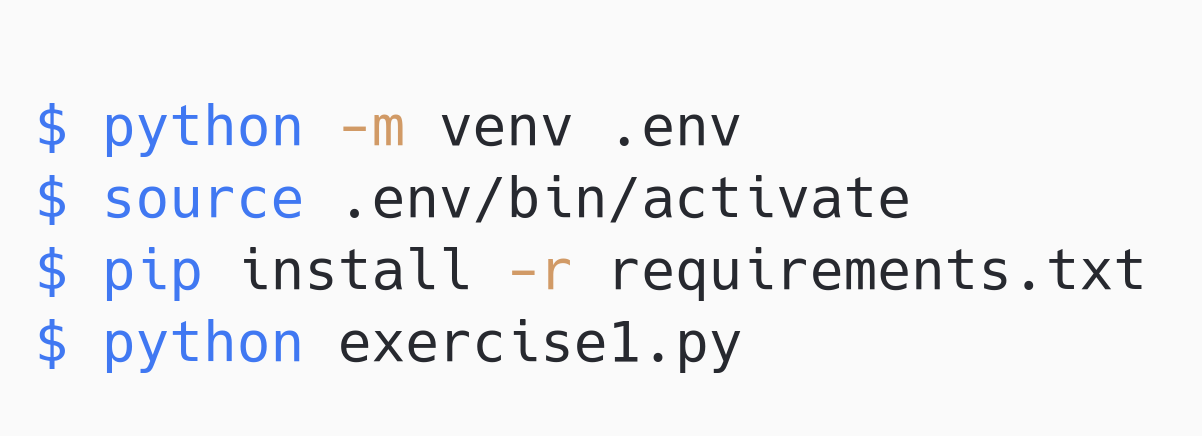
\includegraphics[scale=0.3]{images/exercise1_run.png}
	\caption{Οδηγίες εκτέλεσης προγράμματος}
\end{matlab}

\subsubsection*{Example Usage}

Η οπτικοποίηση του απλού και μικρού train dataset πριν την κανονικοποίηση δίνεται παρακάτω. Για τις δύο κατηγορίες έχουν χρησιμοποιηθεί τα χρώματα μπλε και πράσινο. Ο αλγόριθμος κατηγοριοποιεί τα δύο κόκκινα σημεία. Το ένα ανήκει στην κατηγορία των πράσινων αντικειμένων και το άλλο στην κατηγορία των μπλε αντικειμένων. \\

\begin{matlab}
	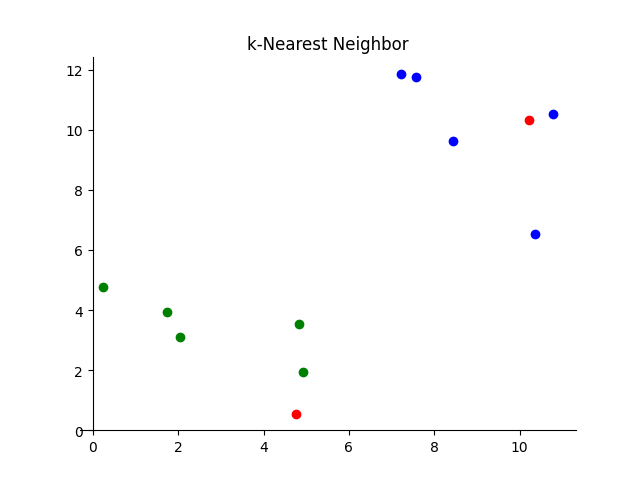
\includegraphics[scale=0.8]{images/exercise1.png}
	\caption{Απλό παράδειγμα κατηγοριοποίησης με k-NN.}
\end{matlab}

\pagebreak

\subsection*{2. Using the code provided at the class (or implementing your own) explain what
	is the curse of dimensionality and how is related to the k-NN algorithm.}

Είναι συχνό φαινόμενο, σε επίπεδο εκμάθησης αλγορίθμων μηχανικής μάθησης ή εξόρυξης δεδομένων, να περιορίζεται η μελέτη σε προβλήματα που ορίζονται πάνω σε λίγες διαστάσεις, Συνήθως μελετώνται προβλήματα στις 2 ή στις 3 διαστάσεις και αυτό είναι εύλογο, διότι μπορούμε πολύ εύκολα να αναπαραστήσουμε οπτικά τα αποτελέσματα των αλγορίθμων. Ωστόσο, στην πραγματικότητα τα προβλήματα ορίζονται σε περισσότερες διαστάσεις από 2 ή 3. \\

Οι διαστάσεις σε ένα πρόβλημα ανάλυσης δεδομένων αντικατοπτρίζουν τα χαρακτηριστικά των αντικειμένων που χρησιμοποιούνται ως βάση για την εκπαίδευση του εκάστοτε αλγορίθμου και ως στόχοι του. Για να γίνει πιο εύκολα κατανοητή η έννοια των χαρακτηριστικών θεωρούμε το εξής παράδειγμα: έστω ότι τα αντικείμενα που επεξεργάζεται ο αλγόριθμος αναπαριστούν τα οχήματα: 'αυτοκίνητο' και 'ποδήλατο' και επιθυμούμε να αποφανθούμε για ένα νέο αντικείμενο αν ανήκει στην κλάση των αυτοκινήτων ή των ποδηλάτων. Τα χαρακτηριστικά που μπορούν να χρησιμοποιηθούν για την περιγραφή των αντικείμενων μπορούν ενδεικτικά να είναι, το πλήθος των τροχών, το μέγεθος, το βάρος κ.α. \\

Φαινεταί λογικό πως όσα περισσότερα χαρακτηριστικά κατέχει το κάθε αντικείμενο, τόσο πιο εύκολο θα είναι για τον αλγόριθμο να προβλέψει σε ποιά κλάση αντικειμένων ανήκει το προς εξέταση αντικείμενο. Ωστόσο, δεν πρέπει να αποκρυφθεί ότι ένα πολύ σημαντικό ζήτημα στην περίπτωση των πολλών χαρακτηριστικών (ή αλλιώς πολλών διαστάσεων) είναι οι μεγάλες απαιτήσεις σε μνήμη, υπολογιστική ισχύ και χρόνο. Πέρα από την ανάκυψη αυτού του πρακτικού ζητήματος, οι πολλές διαστάσεις οδηγούν και σε ένα πολύ σημαντικό πρόβλημα που καλείται "η κατάρα των πολλών διαστάσεων" ή αλλιώς "η κατάρα της διαστατικότητας" (The Curse of Dimensionality). Ο όρος προέκυψε το 1961 από τον Richard E. Bellman. \\

Η κατάρα των πολλών διαστάσεων δεν είναι ένα πρόβλημα που μπορεί να οριστεί αυστηρά σε κάθε αλγόριθμο ανάλυσης δεδομένων. Αυτό συμβαίνει διότι εξαρτάται άμεσα από το σύνολο των δεδομένων και τον εκάστοτε αλγόριθμο. Πιο συγκεκριμένα, το ίδιο μοντέλο μπορεί να παρουσιάζει αρκετά καλή συμπεριφορά, δηλαδή ο αλγόριθμος να δίνει καλό Accuracy, για ένα σύνολο δεδομένων όπου η διάστασή του είναι n και για μεγαλύτερη διάσταση από αυτήν το Accuracy να μειώνεται σημαντικά. Να σημειώσουμε εδω ότι το Accuracy χρησιμοποιείται στους αλγορίθμους μηχανικής μάθησης ως μετρική για την αξιολόγηση του εκάστοτε αλγορίθμου. και δίνεται από τον τύπο

\begin{align*}
	\text{Accuracy} = \frac{\# \text{ correct predictions} }{\# \text{ predictions}}.
\end{align*}

Ουσιαστικά το n είναι ένα threshold για τον συγκεκριμένο αλγόριθμο και τα συγκεκριμένα δεδομένα. Το threshold αυτό δεν είναι ένα σταθερό μέγεθος και μεταβάλεται αναλόγως τον αλγόριθμο και τα δεδομένα. \\ 

Η κατάρα των πολλών διαστάσεων σίγουρα αντιβαίνει στη διαίσθηση που έχει ο άνθρωπος. Θα πίστευε κανείς πως όσα περισσότερα χαρακτηριστικά έχει στη διάθεσή του, τόσο πιο εύκολη θα ήταν η κατηγοριοποίηση των αντικειμένων. Κάτι τέτοιο όμως δε συμβαίνει στην πραγματικότητα. Για να εξηγήσουμε το φαινόμενο αυτό αρχικά θα το περιγράψουμε διαισθητικά και απο τη γεωμετρική σκοπιά των πραγμάτων και στη συνέχεια θα το ορίσουμε με αυστηρά μαθηματικά. \\

Για τη γεωμετρική προσέγγιση του ζητήματος επιστρατεύουμε ξανά το παράδειγμα με τα οχήματα που προαναφέραμε. Για να αποφανθούμε για την κατηγορία οχήματος για κάποιο αντικείμενο που δε γνωρίζουμε την κατηγορία του μία απλή τεχνική είναι να διαμερίσουμε τον χώρο στον οποίο ζουν τα δεδομένα και το καινούριο αντικείμενο να λάβει label ανάλογα με την περιοχή του χώρου στην οποία εντοπίζεται. Αν δηλαδη βρίσκεται σε περιοχή που υπερισχύει η κλάση των ποδηλάτων, δηλαδή σε αυτήν την περιοχή εντοπίζονται περισσότερα ποδήλατα, τότε θα λάβει το label "ποδήλατο" και αντίστοιχα για οποιαδήποτε άλλη κατηγορία οχήματος. \\

Αν αποφασίσουμε τα αντικείμενα να περιγράφονται από ένα χαρακτηριστικό, τότε τα σημεία που αναπαριστούν τα οχήματα τοποθετούνται πάνω σε μία ευθεία. Αν διαιρέσουμε την ευθεία σε ίσα τμήματα, παράγονται m το πλήθος τέτοια τμήματα. Αν ακολουθήσουμε την ίδια διαδικασία στις 2 διαστάσεις, δηλαδή αν τα αντικείμενά μας τώρα περιγράφονται από 2 χαρακτηριστικά, παρατηρούμε ότι τα κελιά που δημιουργούνται, τα οποία έχουν τη μορφή τετραγώνων είναι πολλά περισσότερα σε αριθμό, ενώ στις 3 διαστάσεις η ίδια διαδικασία θα παράξει ίσους κύβους ως κελιά και το πλήθος αυτών θα είναι πολύ μεγαλύτερο σε σχέση με το πλήθος των κελιών στις 2 διαστάσεις και στη 1 διάσταση. \\

\begin{align*}
	\text{πλήθος κελιών στη 1 διάσταση} \ll \text{ πλήθος κελιών στις 2 διαστάσεις} \ll \text{ πλήθος κελιών στις 3 διαστάσεις}
\end{align*}

\begin{matlab}
	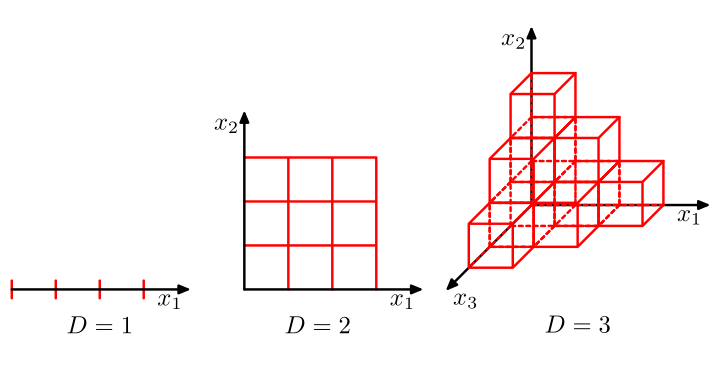
\includegraphics[scale=0.6]{images/cells.png}
	\caption{Διάσπαση του χώρου αναπαράστασης των δεδομένων σε ίσα κελιά, για χώρο διάστασης D = 1, D = 2 και D = 3. Το πλήθος των κελιών αυξάνεται σημαντικά όσο αυξάνεται η διάσταση του χώρου. (πηγή: Pattern Recognition and
Machine Learning, Christopher M. Bishop)}
\end{matlab}

Να επισημάνουμε στο σημείο αυτό, ότι ο όρος "κελί" εδώ χρησιμοποιείται καταχρηστικά και αναφέρεται είτε σε ευθύγραμμο τμήμα, είτε σε τετράγωνο, είτε σε κύβο αναλόγως με το D. \\

Μπορεί κανείς εύκολα να συμπεράνει πώς όσο αυξάνεται το D, δηλαδή το πλήθος των χαρακτηριστικών, τόσα περισσότερα κελιά θα μένουν χωρίς σημεία. Καθώς το πλήθος των δεδομένων είναι σταθερό και καθορισμένο και για τις τρεις διαφορετικές περιπτώσεις D, το ίδιο πλήθος σημείων αντιστοιχεί σε περισσότερα κελιά καθώς το D αυξάνεται. Συνεπώς, όσο αυξάνεται η διάσταση του προβλήματος τόσο τα σημεία διασπείρονται στο χώρο και οι μεταξύ τους αποστάσεις μεγαλώνουν σημαντικά. \\

Η παρατήρηση αυτή μπορεί να επιβεβαιωθεί και πειραματικά. Επιλέξαμε να τρέξουμε τον κώδικα που αφορά την κατάρα της διαστατικότητας που παρουσιάστηκε στο μάθημα και να τον παραμετροποιήσουμε με τέτοιον τρόπο, ώστε να μπορέσουμε να παράξουμε ασφαλή συμπεράσματα σχετικά με το φαινόμενο. Παραθέτουμε παρακάτω τον κώδικα για λόγους διευκόλυνσης του αναγνώστη. \\ 

\begin{lstlisting}
def random_point(dim):
	return [random.random() for _ in range(dim)]

def random_distances(dim, num_pairs):
	return [distance(random_point(dim), random_point(dim))
			for _ in range(num_pairs)]

dimensions = range(1, 10000, 1000)

avg_distances = []
min_distances = []

random.seed(0)

for dim in dimensions:
	distances = random_distances(dim, 10000)  # 10,000 random pairs
	avg_distances.append(mean(distances))     # track the average
	min_distances.append(min(distances))      # track the minimum
	print(f"DIMENSION: {dim} MIN DISTANCE {min(distances)} MEAN DISTANCE: {mean(distances)}")

plt.title('The Curse of Dimensionality') 

plt.plot(dimensions, avg_distances, label = "avg_distances")
plt.plot(dimensions, min_distances, label = "min_distances")

# naming the x axis 
plt.xlabel('dimensions') 
# naming the y axis 
plt.ylabel('distances')

plt.legend()     
plt.show()            
\end{lstlisting}

Τρέξαμε τον κώδικα για διαφορετικό εύρος διαστάσεων και πλήθος σημείων. Ενδεικτικά αποτελέσματα παρουσιάζονται στα διαγράμματα παρακάτω. \\

\begin{matlab}
	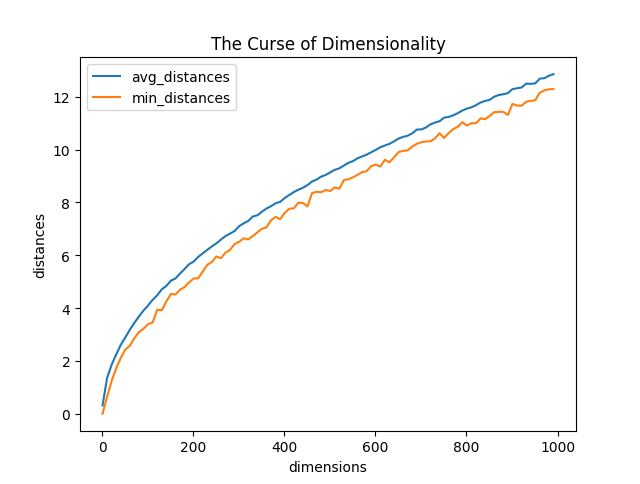
\includegraphics[scale=0.6]{images/the_curse_of_dimensionality_1_to_1000.png}
	\caption{Η κατάρα της διαστατικότητας: αναπαράσταση της μέσης και της ελάχιστης απόστασης δύο σημειών σε χώρους διάστασης από D = 1 εως και D = 1000}
\end{matlab}

\begin{matlab}
	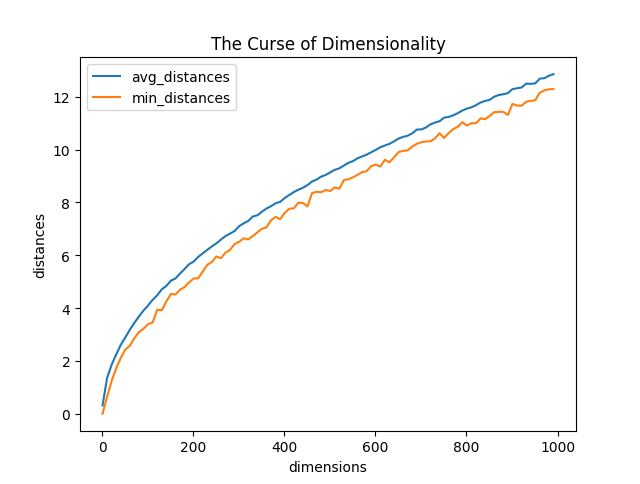
\includegraphics[scale=0.6]{images/the_curse_of_dimensionality_1_to_1000.png}
	\caption{Η κατάρα της διαστατικότητας:  αναπαράσταση της μέσης και της ελάχιστης απόστασης δύο σημειών σε χώρους διάστασης από D = 1 εως και D = 1000}
\end{matlab}

\begin{matlab}
	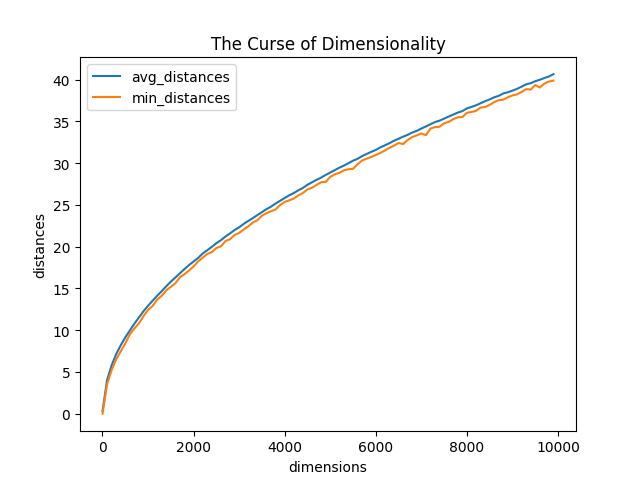
\includegraphics[scale=0.6]{images/the_curse_of_dimensionality_1_to_10000.png}
	\caption{Η κατάρα της διαστατικότητας:  αναπαράσταση της μέσης και της ελάχιστης απόστασης δύο σημειών σε χώρους διάστασης από D = 1 εως και D = 10000}
\end{matlab}

Παρατηρούμε ότι όσο αυξάνεται το πλήθος των χαρακτηριστηκών, τόσο αυξάνεται και η απόσταση των σημείων μεταξύ τους και μάλιστα με πολύ γρήγορο ρυθμό, γεγονός που πιστοποιεί όσα ήδη έχουμε αναφέρει για την κατάρα των πολλών διαστάσεων. Η αύξηση της μέσης απόστασης μεταξύ των σημείων τείνει να εκφυλίσσει την εννοια της απόστασης, πλέον το πόσο απέχουν δύο αντικείμενα δεν επαρκεί για να παραχθούν ασφαλή συμπεράσματα. Όσο μεγαλώνει η διάσταση, τόσο αραιώνει ο χώρος απο σημεία που αναπαριστούν δεδομένα και αυτό μπορεί να οδηγήσει στη σκέψη ότι τα σημεία αυτά μπορεί να μην είναι πλέον αντιπροσωπευτικά του προβλήματος και να μην πρόκειται για σημεία που αναπαριστούν τον "κανόνα", αλλά την εξαίρεση, γεγονός που δυσκολεύει την παραγωγή ορθών συμπερασμάτων. \\

Αφού κατανοήσαμε διαισθητικά και πειραματικά την κατάρας της διαστατικότητας μπορούμε πλέον να περάσουμε στον πιο αυστηρό και με μαθηματικό τρόπο ορισμό του φαινομένου. \\

Αρχικά, πρέπει να αναφέρουμε ορισμένες σημαντικές μαθηματικές έννοιες, για να μπορέσουμε να ορίσουμε το φαινόμενο με αυστηρό τρόπο. Βασιζόμαστε στην ανάλυση και στον συμβολισμό που παρουσιάζεται στο \cite{machinelearning} \\

Στην περίπτωση του 1-ΝΝ, θεωρούμε ότι τα σημεία που αποτελούν το σύνολο εκπαίδευσης ανήκουν στον χώρο \(X\), για τον οποίον ισχύει χωρίς βλάβη της γενικότητας ότι 

\begin{align*}
	X = [0,1]^d
\end{align*}

, όπου \(d\) είναι η διάσταση του χώρου (\(d = 1, 2, ....\)). Ο χώρος \(X\) είναι εξοπλισμένος με μία μετρική \(ρ\), για την οποία ισχύει 

\begin{align*}
	ρ:X \times X \rightarrow \R
\end{align*} 

και η οποία  ακολουθεί μερικούς κανόνες:

\begin{align*}
	\bullet ρ(x,x') &\geq 0 \text{ } \forall x,x' &\text{ Θετικότητα (Positivity)} \\
	\bullet ρ(x,x') &= 0 \Leftrightarrow x = x' &\text{ Θετικότητα (Positivity)} \\
	\bullet ρ(x,x') &= ρ(x',x) &\text{ Συμμετρία (Symmetry)}\\
	\bullet ρ(x,x') &\leq ρ(x,x'') + ρ(x'',x')  \text{ } \forall x,x',x'' &\text{ Τριγωνική Ανισότητα (Triangle Inequality)}
\end{align*}

Μία τέτοια μετρική είναι η Ευκλείδια απόσταση:

\begin{align*}
	ρ(x,x') = \norm{x- x'} =\sqrt{\sum_{i=1}^{d}(x_i - x_{i}')^2}
\end{align*}

Υιοθετούμε την ευκλέιδια απόσταση ως μετρική σε αυτήν την περίπτωση. Τα labels, δηλαδή οι κατηγορίες που αποδίδονται σε κάθε αντικείμενο ανήκουν στον χώρο \(Y\), για τον οποίο ισχύει χωρίς βλάβη της γενικότητας ότι 

\begin{align*}
	Y = [0,1]
\end{align*}   


Θεωρούμε σύνολο \(S\) τέτοιο ώστε 

\begin{align*}
	S = \left\{(x_1, y_1), ...., (x_m, y_m)\right\}
\end{align*}

Με \(m\) συμβολίζεται το πλήθος των αντικειμένων του συνόλου εκπαίδευσης \(S\) του αλγορίθμου. Έστω \(D\) μία κατανομή στο \(X \times Y\) και \(η\) μία συνάρτηση για την οποία ισχύει ότι

\begin{align*}
	η: \R^d \rightarrow \R
\end{align*}

και εκφράζει την πιθανότητα 

\begin{align*}
	η(x) = P[y = 1 | x]
\end{align*}

Η \(η\) είναι c-Lipschitz συνάρτηση, δηλαδή ισχύει ότι υπάρχει κάποια σταθερά c, τέτοια ώστε

\begin{align*}
	|η(x) - η{x'}| \leq c \norm{x-x'}
\end{align*}  

Αν με \(h_s\) συμβολίζουμε τον κανόνα που έχουμε επιλέξει για την αξιολόγηση των σημείων, με \(h_{s}^*\) τον βέλτιστο κανόνα αξιολόγησης σημείων και με \(L_D\) το λάθος ενός κανόνα, είτε αυτός είναι ο \(h\), είτε ο \(h^*\), τότε το αναμενόμενο λάθος στον 1-NN αλγόριθμο φράσσεται ως εξής:

\begin{align*}
	E[L_D(h_s)] \leq 2 L_D(h^*) + 4c \sqrt{d} m^{- \frac{1}{d+1}}
\end{align*} 

Στην περίπτωση όπου \(k \geq 2\), το αντίστοιχο άνω φράγμα γίνεται 

\begin{align*}
	E[L_D(h_s)] \leq (1 + \sqrt{\frac{8}{k}}) L_D(h^*) + (6c \sqrt{d} + k) m^{- \frac{1}{d+1}}
\end{align*} 

Συνεπώς, το σφάλμα που παράγεται από τον αλγόριθμο (ανεξάρτητα από την επιλογή του \(k\)) εξαρτάται από τις ιδιότητες της κατανομης και το m, δηλαδή το πλήθος των αντικειμένων εκπαίδευσης του αλγορίθμου. Ιδανικά, το σφάλμα θέλουμε να είναι μικρότερο από μία μικρή ποσότητα \(ε\). Για να συμβεί αυτό πρέπει

\begin{align*}
	E[L_D(h_s)] \leq ε
\end{align*}

Στην περίπτωση του 1-ΝΝ

\begin{align*}
	4c \sqrt{d} m^{- \frac{1}{d+1}} &\leq ε \Leftrightarrow \\
	m^{- \frac{1}{d+1}} &\leq \frac{ε}{4c \sqrt{d}} \Leftrightarrow \\
	\frac{1}{m^{\frac{1}{d+1}}} &\leq \frac{ε}{4c \sqrt{d}} \Leftrightarrow \\
	m^{\frac{1}{d+1}} &\geq \frac{4c \sqrt{d} }{ε}\Leftrightarrow \\
	\sqrt[d+1]{m} &\geq \frac{4c \sqrt{d} }{ε} \Leftrightarrow \\
	m &\geq \frac{4c \sqrt{d}}{ε}^{d+1} 
\end{align*}

Στην περίπτωση του k-ΝΝ, με \(k \geq 2\)

\begin{align*}
	(6c \sqrt{d} +k) m^{- \frac{1}{d+1}} &\leq ε \Leftrightarrow \\
	m^{- \frac{1}{d+1}} &\leq \frac{ε}{6c \sqrt{d} + k} \Leftrightarrow \\
	\frac{1}{m^{\frac{1}{d+1}}} &\leq \frac{ε}{6c \sqrt{d} + k} \Leftrightarrow \\
	m^{\frac{1}{d+1}} &\geq \frac{6c \sqrt{d} + k }{ε}\Leftrightarrow \\
	\sqrt[d+1]{m} &\geq \frac{6c \sqrt{d} + k }{ε} \Leftrightarrow \\
	m &\geq \frac{6c \sqrt{d} + k}{ε}^{d+1} 
\end{align*}

Συνεπώς, το πλήθος των αντικειμένων που απαρτίζουν το σύνολο εκπαίδευσης του k-NN πρέπει να αυξάνεται εκθετικά με βάση τη διάσταση του χώρου στον οποίον ανήκει το σύνολο των αντικειμένων που εξετάζονται, ώστε ο αλγόριθμος να παράγει ασφαλή αποτελέσματα. Αυτή η εκθετική εξάρτηση του αλγορίθμου από τη διάσταση είναι η κατάρα της διαστατικότητας. \\ 

Παραθέτουμε ενδεικτικά στους παρακάτω πίνακες το μέγεθος ενός συνόλου εκπαίδευσης που χρειάζεται ο k-NN, για να παράξει σωστά αποτελέσματα. Το  \(c\) εδώ είναι 2 και το \(ε\) ισούται με 0.8 \\

\begin{tabular}{ |p{8cm}|p{8cm}|  }
	\hline
	\multicolumn{2}{|c|}{1-NN} \\
	\hline
	Διάσταση Χώρου Συνόλου Εκπαίδευσης (d) & Πλήθος Σημείων Συνόλου Εκπαίδευσης (m)\\
	\hline
	1   & 100    \\
	3   & 83521    \\
	5   & 113379904    \\
	7   & 208827064576    \\
	9   & 590490000000000    \\
	\hline
\end{tabular}
 
\medspace
 
\begin{tabular}{ |p{8cm}|p{8cm}|  }
	\hline
	\multicolumn{2}{|c|}{3-NN} \\
	\hline
	Διάσταση Χώρου Συνόλου Εκπαίδευσης (d) & Πλήθος Σημείων Συνόλου Εκπαίδευσης (m)\\
	\hline
	1   & 225    \\
	3   & 331776    \\
	5   & 729000000    \\
	7   & 2251875390625    \\
	9   & 8140406085191601    \\
	\hline
\end{tabular}

\medspace

\begin{tabular}{ |p{8cm}|p{8cm}|  }
	\hline
	\multicolumn{2}{|c|}{10-NN} \\
	\hline
	Διάσταση Χώρου Συνόλου Εκπαίδευσης (d) & Πλήθος Σημείων Συνόλου Εκπαίδευσης (m)\\
	\hline
	1   & 576    \\
	3   & 1185921    \\
	5   & 3518743761    \\
	7   & 14048223625216    \\
	9   & 64925062108545024    \\
	\hline
\end{tabular}

\medspace

Ο υπολογισμός των τιμών που παρουσιάζονται στους παρακάτω πίνακες έγινε με βάση το πρόγραμμα που βρίσκεται στο αρχείο number\_of\_points.py. \\

\begin{lstlisting}
import math

dimensions = range(1, 10, 2)

c = 2
e = 0.8

print("1-NN")
for dim in dimensions:
	frac = int(4 * c * math.sqrt(dim) / e)
	points = pow(frac, dim + 1)
	print(f"Dimension: {dim} points: {points}")

print("k-NN")
neighboors = range(2, 11, 1)
for k in neighboors:
	for dim in dimensions:
		frac = int((6 * c * math.sqrt(dim)) + k / e)
		points = pow(frac, dim + 1)
		print(f"k = {k} Dimension: {dim} points: {points}")            
\end{lstlisting}

Θα μπορούσε κανείς να υποστηρίξει ότι η κατάρα της διαστατικότητας μπορεί να αντιμετωπιστεί με την προσθήκη κάθε φορά όλων των απαραίτητων σημείων, ώστε ο αλγόριθμος να παράγει ασφαλή αποτελέσματα. Ωστόσο, αυτή δεν είναι μία αποδοτική λύση, καθώς το πλήθος των σημείων που θα χρειάζεται κάθε φορά ο αλφόριθμος θα αυξάνεται εκθετικά σύμφωνα με τη διάσταση του χώρου των αντικειμένων. Συνεπώς, μία πιο ασφαλής προσέγγιση του ζητήματος είναι να περιορίσουμε τις διαστάσεις, δηλαδή τα χαρακτηριστικά των αντικειμένων. Δεν είναι πάντοτε όλα τα χαρακτηριστικά σημαντικά για την εξαγωγή συμπερασμάτων στη μηχανική μάθηση. Οι διαστάσεις μπορούν να μειωθούν με διάφορους τρόπους (ενδεικτικά παραδείγματα αποτελούν τα PCA και SVD, που είναι κλασσικές τεχνικές στην μηχανική μάθηση), έτσι ώστε ο αλγόριθμος να μην αντιμετωπίζει πρόβλημα ως προς τη διάσταση και τα δεοδμένα. 

\pagebreak

\subsection*{3. \\ 1. Suppose there is a set of points on a two-dimensional plane from two different classes.
	Points in class Red are (0, 1), (2, 3), (4, 4) and points in class Blue are (2, 0), (5, 2),
	(6, 3). Draw the k-nearest-neighbor decision boundary for k = 1 as we discussed in the
	lecture. Experiment yourself with two or more differrent distance metrics. Present your
	results. \\
	2. If the y-coordinate of each point was multiplied by 5, what would happen to the k =
	1 boundary? Draw a new picture. Explain whether this effect might cause problems in
	practice.
\\
	3. Can you draw the decision boundary for k=3?
\\
	4. Suppose now we have a test point at (1, 2). How would it be classied under 3-NN? Given
	that you can modify the 3-NN decision boundary by adding points to the training set in
	the diagram, what is the minimum number of points that you need to add to change the
	classication at (1, 2)? Provide also the coordinates for these new points and justify your
	answer.}

\pagebreak

\subsection*{4. How long does it take for k-NN to classify one point? Or in other words
	what is the testing complexity for one instance? Assume your data has dimensionality d, you
	have n training examples and use Euclidean distance. Assume also that you use a quick select
	implementation which gives you the k smallest elements of a list of length m in O(m).}


\pagebreak

\subsection*{5. To see an application of the k-NN algorithm in a real world classification prob-
	lem consider the data found at https://www.kaggle.com/uciml/iris. Download from there the
	Iris.csv file. Ignore the id column and consider the columns: SepalLengthCm, SepalWidthCm,
	PetalLengthCm, PetalWidthCm as point coordinates in a four dimensional space. Consider the
	column Species as the class/label column. The file contains 150 rows. Run the algorithm on
	the first 100 rows and make predictions for the rest 50. How your predictions are compared to
	the actual? Explain your methodology.}

\pagebreak

\begin{thebibliography}{9}
	\bibitem{machinelearning} 
	Understanding Machine Learning: From Theory to Algorithms, 
	Shai Shalev-Shwartz and Shai Ben-David,
	Cambridge University Press, 2014,
	pages. 258-267, 
	ISBN: 978-1-107-05713-5
	
	\bibitem{dimreduction} 
	Πολύτροπη Μείωση Διάστασης Δεδομένων με Χρήση Πυρήνα,
	Διπλωματική εργασία, 
	Πέτρος Χ. Δρακούλης,
	Αριστοτέλειο Πανεπιστήμιο Θεσσαλονίκης, Τμήμα ΠΛηροφορικής, 2016
	
	\bibitem{dimreduction} 
	Pattern recognition and machine learning, 	
	Christopher Bishop,
	Springer, 2006,
	pages. 33-38, 
	ISBN: 978-0-387-31073-2
	
\end{thebibliography}

\end{document}
